\chapter{Caso de estudio: Sistema de climatización}
\label{chap:caso_estudio}

Para validar la arquitectura definida, decidimos implementar un pequeño sistema autoadaptativo. Se trata de un sistema de climatización que gestiona la temperatura de una habitación. En este capítulo especificaremos sus componentes y describiremos su desarrollo. Nos servirá como aplicación de referencia para guiar el diseño de futuras soluciones.

\section{Análisis}

El primer paso fue capturar los requisitos del sistema a implementar. Cómo se ha comentado, queremos desarrollar un sistema de climatización. Este sistema regulará la temperatura de una habitación mediante el uso de un \textbf{aparato de aire acondicionado}. Este ofrece \textbf{tres modos de funcionamiento}: un modo para calentar la estancia, otro para enfriarla, y un estado neutral (apagado). Además, cuenta con un \textbf{termómetro} interno que nos reporta la temperatura periódicamente.

\begin{figure}[h!]
  \centering
  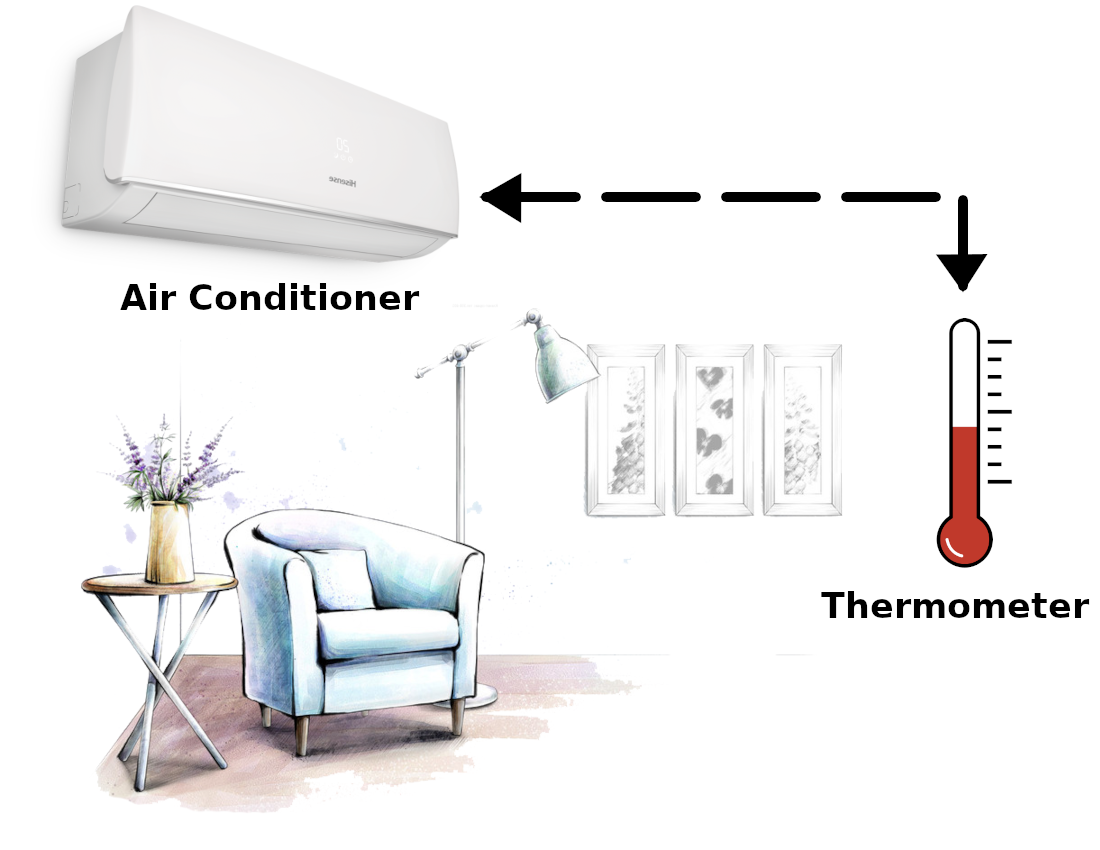
\includegraphics[scale=0.20]{cap_caso-estudio/images/aire-acondicionado}
  \caption[Diagrama básico del sistema de climatización. Aparecen los componentes principales: el aire acondicionado y el termómetro.]{Diagrama básico del sistema de climatización. Aparecen los componentes principales: el aire acondicionado y el termómetro. \footnotemark}
  \label{fig:caso-estudio-diagrama}
\end{figure}

\footnotetext{Imágenes originales obtenidas de: \href{https://freesvg.org/temperatur}{termómetro}, \href{https://pngimg.com/image/45204}{aire acondicionado} y \href{https://www.pngall.com/home-interior-design-png/download/50368}{salón}.}

Para poder climatizar la habitación, necesitamos que el usuario defina su temperatura objetivo: la \textbf{temperatura de confort}. Cambios en la temperatura de la estancia deberán activar o desactivar el aparato para alcanzarla. Es importante evitar que el aire acondicionado se encienda y se apague constantemente cuando esta se alcance o sobrepase. Por ello, usaremos unas \textbf{temperaturas umbrales}. Por ejemplo, $\pm 4$ºc respecto a la temperatura de confort.

\section{Diseño}

Del análisis anterior ya podemos deducir la existencia de dos componentes: un aparato de aire acondicionado (el recurso manejado) y un termómetro (la sonda). Aparte de ellos, deberemos implementar la infraestructura necesaria para completar bucle MAPE-K: monitores, módulos de reglas y efectores que nos permitan interactuar con el sistema manejado.

Para describir su diseño usaremos la notación de sistemas autoadaptativos descrita en \cite{fonsEspecificacionSistemasAutoadaptativos2021}:

\subsection{Sondas:}

Para implementar el sistema, requerimos de las siguientes sondas:

\begin{longtable}{|r p{11.5cm}|}
    \hline
    \textbf{Sonda:} & \texttt{thermometer}  \\
    \textbf{Descripción:} & Reporta la temperatura actual de la habitación (en ºc). \\
    \textbf{Monitor:} & \texttt{Climatisation.Monitor} \\
    \textbf{Datos:} & \texttt{temperature} \\
    \hline
    \textbf{Sonda:} & \texttt{airconditioner-mode-changed-probe}  \\
    \textbf{Descripción:} & Reporta el modo de funcionamiento del aire acondicionado cuando este cambia. \\
    \textbf{Monitor:} & \texttt{Climatisation.Monitor} \\
    \textbf{Datos:} & \texttt{airconditioner-mode} \\
    \hline
    \textbf{Sonda:} & \texttt{airconditioner-adaption-loop-registration}  \\
    \textbf{Descripción:} & Cuando el servicio de aire acondicionado se inicia, registra la configuración inicial del sistema. \\
    \textbf{Monitor:} & \texttt{Climatisation.Monitor} \\
    \textbf{Datos:} &  \ttfamily\selectfont airconditioner.is-deployed, airconditioner-mode, target-temperature,cold-temperature-threshold, hot-temperature-threshold \\
    \hline

    \caption{Sondas del sistema de climatización.}
    \label{tab:climatisation-probes}
\end{longtable}

\subsection{Propiedades de adaptación:}

También podemos deducir cuáles son nuestras propiedades de adaptación:

\begin{longtable}{|r p{11.5cm}|}
    \hline
    \textbf{Propiedad:} & \texttt{temperature}  \\
    \textbf{Descripción:} & Representa la temperatura actual de la habitación (en ºC).  \\
    \textbf{Tipo de dato:} & \texttt{float} \\
    \hline
    \textbf{Propiedad:} & \texttt{target-temperature}  \\
    \textbf{Descripción:} & La temperatura de confort definida por el usuario. El sistema deberá adaptarse para alcanzarla.  \\
    \textbf{Tipo de dato:} & \texttt{float} \\
    \hline
    \pagebreak
    \hline
    \textbf{Propiedad:} & \texttt{cold-temperature-threshold}  \\
    \textbf{Descripción:} & La temperatura umbral de frío (en ºc). Si la temperatura baja por debajo de este umbral, deberá calentarse la habitación. \\
    \textbf{Tipo de dato:} & \texttt{float} \\
    \hline
    \textbf{Propiedad:} & \texttt{hot-temperature-threshold}  \\
    \textbf{Descripción:} & La temperatura umbral de calor (en ºc). Si la temperatura sube por encima de este umbral, deberá enfriarse la habitación. \\
    \textbf{Tipo de dato:} & \texttt{float} \\
    \hline
    \textbf{Propiedad:} & \texttt{airconditioner.is-deployed}  \\
    \textbf{Descripción:} & Indica si el servicio de aire acondicionado está desplegado y en funcionamiento.  \\
    \textbf{Tipo de dato:} & \texttt{bool} \\
    \hline
    \textbf{Propiedad:} & \texttt{airconditioner-mode}  \\
    \textbf{Descripción:} & Representa el modo de operación actual del aire acondicionado.\linebreak Valores: \texttt{Off} = 0, \texttt{Cooling} = 1, \texttt{Heating} = 2  \\
    \textbf{Tipo de dato:} & Enumerado \\
    \hline

  \caption{Propiedades de adaptación del sistema de climatización.}
  \label{tab:climatisation-adaption-properties}
\end{longtable}

\subsection{Monitores:}

Se necesita definir los monitores que capturarán los datos de las sondas. Estos deberán procesar las mediciones, agregarlas y filtrarlas. De esta forma, detectaremos si hubiera errores de medición, datos obsoletos, etc. Así se evitará que se lleve a cabo adaptaciones incorrectas.

Tomemos el monitor de las temperaturas \texttt{climatisation.monitor.temperature}. Este valida que la nueva medida de temperatura esté a menos de 5ºc de diferencia; o haya más de un minuto de diferencia entre ellas. Como en el ejemplo se trabajó con un aire acondicionado ficticio, se estableció un margen de error grande. Si no cumple una de estas condiciones, será descartada. Así evitamos que el aire acondicionado se active o desactive por un error de medición.

\begin{longtable}{|p{3cm} p{10.9cm}|}
    \hline

    \textbf{Monitor:} & \texttt{climatisation.monitor.temperature}  \\
    \textbf{Descripción:} & Recibe los reportes de temperatura de los termómetros. También filtra estos datos para detectar casos donde se sospecha un error de lectura. \\
    \textbf{Actualiza \linebreak propiedades:} & \linebreak \texttt{temperature} \\
    \multirow{3}*{\textbf{Acciones:}}
        & \linebreak \textbf{SI} $|$\texttt{new-temperature} $-$ \texttt{temperature}$| \le 5.0$ \\
        & \textbf{O} \texttt{request.DateTime} $-$ \texttt{previousMeasurement.DateTime} $>$ 60s \\
        & \textbf{ACTUALIZA-KNOWLEDGE} \texttt{temperature} $=$ \texttt{new-temperature} \\
    \hline

    \textbf{Monitor:} & \texttt{climatisation.monitor.configuration}  \\
    \textbf{Descripción:} & Recibe la configuración del aire acondicionado y la registra en el \texttt{knowledge}. \\
    \textbf{Actualiza \linebreak propiedades:} & \linebreak \ttfamily\selectfont airconditioner.is-deployed, airconditioner-mode, target-temperature, cold-temperature-threshold, hot-temperature-threshold \\

    \pagebreak

    \multirow{2}*{\textbf{Acciones:}}
        & \linebreak \textbf{SI} \texttt{property} $\neq$ \texttt{new-value} \\
        & \textbf{ACTUALIZA-KNOWLEDGE} \texttt{property} $=$ \texttt{new-value} \\
    \hline

  \caption{Monitores del bucle MAPE-K del sistema de climatización.}
  \label{tab:climatisation-monitors}
\end{longtable}

\subsection{Reglas de adaptación}
\label{sec:caso-estudio-diseño-reglas}

Las reglas de adaptación del sistema deberán activar o desactivar el aire acondicionado en base a la temperatura actual. Por ejemplo, si la temperatura es inferior al umbral de frío, el aparato se enciende en modo calefacción. Las reglas se ubicarán en el servicio \texttt{Climatisation.Rules.Service}. Se dispararán cuando cambie uno de sus parámetros.

En la tabla \ref{tab:adaption-rules-climatisation} especificamos las cuatro reglas necesarias. Como comentamos en el capítulo anterior, en el prototipo implementado del bucle MAPE-K nos limitamos a implementar las adaptaciones de tipo \foreign{english}{set parameter}. Por tanto, no definiremos ninguna regla con adaptaciones de despliegue o de \foreign{english}{binding}.

\begin{longtable}{|r p{12.8cm}|}
    \hline
    \textbf{Regla:} & \emph{EnableAirConditionerHeatingModeWhenColdTemperatureThresholdExceeded}  \\
    \textbf{Descripción:} & Activa el aire acondicionado en modo calefacción cuando la temperatura sea inferior al umbral de frío.  \\
    \textbf{Condición:} & \emph{airconditioner-mode} $\neq$ \emph{Heating} \textbf{AND} \emph{temperature} $\le$ \emph{cold-temperature-threshold}  \\
    \textbf{Cuerpo:}   &  \\
    & 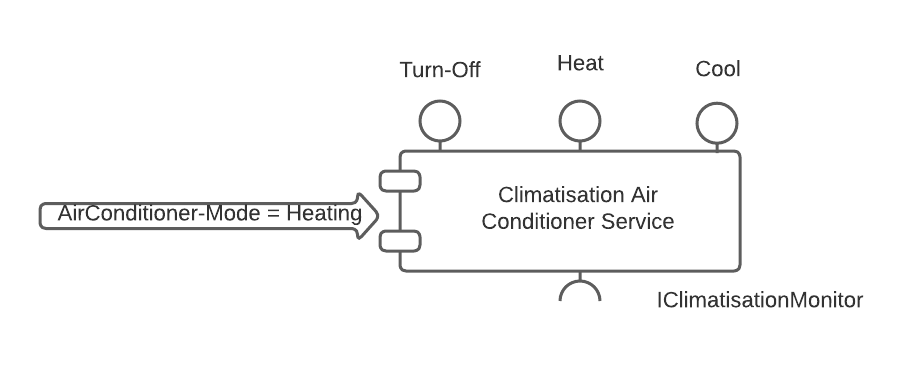
\includegraphics[scale=0.75]{cap_caso-estudio/images/adaption-loop-rule-heat} \\
    \hline

    \textbf{Regla:} & \emph{DisableAirConditionerWhenHeatingModeEnabledAndTargetTemperatureReached}  \\
    \textbf{Descripción:} & Apaga el aire acondicionado cuando el modo calefacción está activo y se ha alcanzado la temperatura de confort.  \\
    \textbf{Condición:} & \emph{airconditioner-mode} $=$ \emph{Heating} \textbf{AND} \emph{temperature} $\ge$ \emph{target-temperature}  \\
    \textbf{Cuerpo:} &  \\
    & 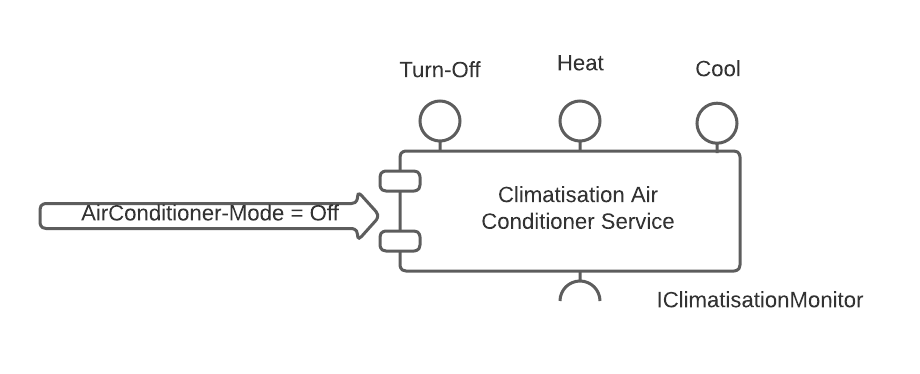
\includegraphics[scale=0.75]{cap_caso-estudio/images/adaption-loop-rule-off} \\
    \hline

    \textbf{Regla:} & \emph{EnableAirConditionerCoolingModeWhenTemperatureThresholdExceeded}  \\
    \textbf{Descripción:} & Activa el aire acondicionado en modo enfriar cuando la temperatura sea superior al umbral de calor.  \\
    \textbf{Condición:} & \emph{airconditioner-mode} $\neq$ \emph{Cooling} \textbf{AND} \emph{temperature} $\ge$ \emph{hot-temperature-threshold}  \\
    \pagebreak
    \textbf{Cuerpo:} &  \\
    & 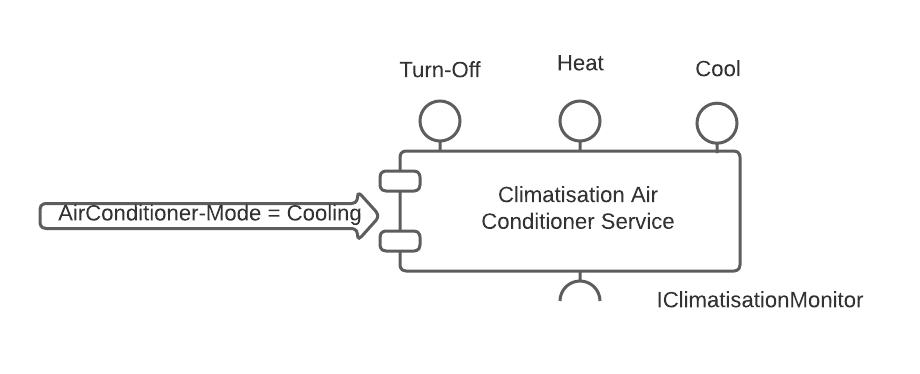
\includegraphics[scale=0.75]{cap_caso-estudio/images/adaption-loop-rule-cooling} \\
    \hline

    \textbf{Regla:} & \emph{DisableAirConditionerWhenCoolingAndTargetTemperatureReachedAdaptionRule}  \\
    \textbf{Descripción:} & Apaga el aire acondicionado cuando el modo enfiar está activo y se ha alcanzado la temperatura de confort.  \\
    \textbf{Condición:} & \emph{airconditioner-mode} $=$  \emph{Cooling} \textbf{AND} \emph{temperature} $\le$ \emph{target-temperature}  \\
    \textbf{Cuerpo:} &  \\
    & 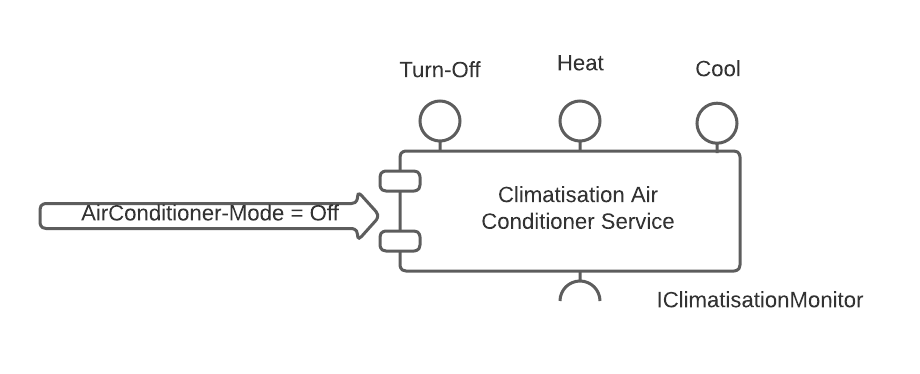
\includegraphics[scale=0.75]{cap_caso-estudio/images/adaption-loop-rule-off} \\
    \hline

  \caption{Reglas de adaptación del sistema de climatización.}
  \label{tab:adaption-rules-climatisation}
\end{longtable}

\subsection{Efectores:}

Los efectores que expondrá el aire acondicionado para cambiar su modo de funcionamiento son:

\begin{table}[htb]
  \centering

  \begin{tabular}{|r p{11.5cm}|}
    \hline
    \textbf{Efector:} & \emph{airconditioner.heat}  \\
    \textbf{Descripción:} & Activa el modo calentar del aire acondicionado. \\
    \hline
    \textbf{Efector:} & \emph{airconditioner.cool}  \\
    \textbf{Descripción:} & Activa el modo enfriar del aire acondicionado. \\
    \hline
    \textbf{Efector:} & \emph{airconditioner.turn-off}  \\
    \textbf{Descripción:} & Apaga el aire acondicionado. \\
    \hline
  \end{tabular}

  \caption{Efectores del sistema de climatización.}
    \label{tab:climatisation-effectors}
\end{table}

\section{Implementación}

En esta sección describiremos la implementación del sistema de climatización. Para funcionar como un elemento autónomo, tendremos que emplear los servicios del bucle MAPE-K distribuido y otros cuatro nuevos. Por un lado, estará el recurso manejado, el aire acondicionado. Y por el otro, tendremos los servicios de infraestructura necesarios para operar con el bucle. Estos son el monitor, el servicio de reglas y el servicio de efectores.

Para su implementación, hemos empleado las mismas tecnologías descritas en el capítulo \ref{chap:implementación}: microservicios \texttt{ASP.NET}, comunicación mediante APIs REST basadas en HTTP y \foreign{english}{brokers} de mensajería \texttt{RabbitMQ}. A continuación, describiremos cada uno:

\subsection{Servicio de aire acondicionado}

El servicio de aire acondicionado será nuestro recurso manejado. Este cuenta con tres modos de operación: apagado (\texttt{OFF}), enfriando (\texttt{COOLING}) o calentando (\texttt{HEATING}). Según el modo, simulará el aumento o disminución de la temperatura que reporta el termómetro interno. Incluso cuando esté apagado, la temperatura variará para forzar su activación. De esta forma, podemos verificar más rápido si se aplican correctamente las adaptaciones.

El componente expone una API con tres \foreign{english}{endpoints} para cambiar el modo. Son estos los que invocará el ejecutor durante las adaptaciones. Además, cuando se produzca el cambio, reportará automáticamente al monitor su nuevo valor. Esto servirá para confirmar el cambio y completar el proceso de adaptación.

El termómetro interno está implementado como un servicio en segundo plano dentro del aire acondicionado. Un \foreign{english}{background service}\footnote{Documentación oficial: \url{https://docs.microsoft.com/en-us/aspnet/core/fundamentals/host/hosted-services\#backgroundservice-base-class}} de ASP.NET. Este reportará periódicamente, cada pocos segundos, la temperatura actual al monitor.

Durante el arranque del servicio tenemos otra tarea en segundo plano. Esta se ejecuta una sola vez y se encarga de registrar la configuración inicial del recurso manejado. Este dará valor a las propiedades como los umbrales de temperatura o las variables como \texttt{is-deployed} en el conocimiento.

\subsection{Monitor}

El monitor de la solución expone un \foreign{english}{endpoint} para recabar las mediciones de temperatura. Se encuentra en la ruta \texttt{POST Measurement/Temperature}. Cuando reciba un valor deberá validarlo. El monitor descartará aquellos con diferencias mayores a 5ºC y tomados con menos de un minuto de diferencia. En cambio, si es válido, lo envía al servicio de monitorización. Este lo recibirá y lo almacenará en el conocimiento como una propiedad de adaptación.

El servicio también ofrece \foreign{english}{endpoints} para actualizar la configuración del aire acondicionado en el conocimiento. Así podrá registrar su configuración inicial o los modos de operación cuando cambien. Son un subconjunto de los que ofrece el conocimiento, expuestos a través del servicio de monitorización del bucle.

\subsection{Reglas}

En cuanto al servicio de reglas, este contiene las cuatro definidas en el apartado \ref{sec:caso-estudio-diseño-reglas}. Las reglas activan o desactivan el aire acondicionado en base a la temperatura de la estancia. Se han implementado siguiendo la estructura descrita en el apartado \ref{sec:implementacion-modulo-reglas}. Todas ellas heredan de la clase abstracta \texttt{AdaptionRuleBase}. Deben implementar los métodos para evaluar la condición y ejecutar su acción. También tendrán que declarar las propiedades de adaptación de las que dependen para suscribirse a sus cambios.

\pagebreak

Para describirlas tomaremos como ejemplo la regla \texttt{Disable Air Conditioner When Cooling And Target Temperature Reached Adaption Rule}. Esta desactiva el aparato cuando está activo el modo enfriamiento y se ha alcanzado la temperatura de confort. A lo largo de la memoria ya hemos mostrado algunos fragmentos de su código.

La regla describe las propiedades o configuraciones de las que depende mediante atributos. Son los parámetros que requiere para evaluar su condición. Tomemos por ejemplo el fragmento \ref{ls:adaption-rule-dependencies}. Observamos que declara tres dependencias: \texttt{airconditioner-mode}, \texttt{temperature} y \texttt{hot-temperature-threshold}.

En cuanto a la implementación, ya habíamos discutido anteriormente su método \texttt{Execute} en el fragmento \ref{ls:change-request-builder}. Solo nos queda exponer la implementación de referencia del método \texttt{Evaluate}. En el fragmento \ref{ls:adaption-rule-evaluate-condition} podemos ver la condición. Observamos que en las líneas 3-5, 12-15 y 17-20 se obtienen las propiedades de adaptación o claves de configuración desde el servicio de análisis. En base a ellas, en las líneas 22-23 se evalúa.

\begin{lstlisting}[caption={Implementación de referencia del método \texttt{Evaluate}. La regla obtiene del conocimiento el estado actual del sistema y determina si debe ejecutarse.\protect\footnotemark},captionpos=b, label=ls:adaption-rule-evaluate-condition]
protected override async Task<bool> Evaluate()
{
  var currentTemperature =
    await _propertyService.GetProperty<TemperatureMeasurementDTO>(
      ClimatisationConstants.Property.Temperature);

  if (currentTemperature is null)
  {
      return false;
  }

  var airConditionerMode = await _configurationService
    .GetConfigurationKey<AirConditioningMode?>(
        ClimatisationAirConditionerConstants.AppName,
        ClimatisationAirConditionerConstants.Configuration.Mode);

  var targetTemperature = await _configurationService
      .GetConfigurationKey<float?>(
        ClimatisationAirConditionerConstants.AppName,
        ClimatisationConstants.Configuration.TargetTemperature);

  return airConditionerMode == AirConditioningMode.Cooling
      && currentTemperature.Value <= targetTemperature;
}
\end{lstlisting}

\footnotetext{Código disponible \href{https://github.com/Starkie/TFM-DistributedAutoadaptiveSystems/blob/3300a2e54ce0fe82701d53c3d3cb6cbcd64141be/src/AutoAdaptativeSystem/Climatisation/Rules/EventHandlers/Rules/DisableAirConditionerWhenCoolingModeEnabledAndTargetTemperatureAchievedRule.cs\#L51-L72}{aquí}.}

\subsection{Ejecutores}

Finalmente, tenemos el servicio de ejecutores. En la última etapa del bucle de adaptación, el módulo de ejecución emite una notificación con las acciones de adaptación que debe ejecutarse para determinado componente del recurso manejado. El servicio de ejecutores se suscribirá a estas notificaciones de aquellos componentes que gestiona. En este caso, las referentes al aire acondicionado.

Para el caso de estudio, por restricciones de tiempo, nos limitamos a implementar las adaptaciones que implicaban cambios en la configuración del sistema manejado (adaptaciones \foreign{english}{set parameter}). Los efectores que exponga el recurso manejado determinará cómo se ejecutarán estas acciones.

Para el servicio de aire acondicionado, cambiar el modo de operación supone invocar a los \foreign{english}{endpoints} HTTP que expone. En el fragmento \ref{ls:effector-airconditioner-set-parameter} mostramos cómo se ejecuta la acción de adaptación para cambiar la configuración \texttt{Mode}. En base al nuevo valor, se invocará a un \foreign{english}{endpoint} u otro (líneas 14 a 27). Para ello, empleamos el API \foreign{english}{client} generado del servicio de aire acondicionado.

\begin{lstlisting}[caption={Implementación de los efectores del aire acondicionado. Invocan a los endpoints HTTP en base a las acciones de adaptación.\protect\footnotemark},captionpos=b, label=ls:effector-airconditioner-set-parameter]
public async Task<Unit> Handle(
  SetAirConditionerModeRequest notification,
  CancellationToken cancellationToken)
{
    var succeeded = Enum.TryParse(
      notification.Value,
      out AirConditioningMode mode);

    if (!succeeded)
    {
        return Unit.Value;
    }

    switch (mode)
    {
        case AirConditioningMode.Off:
            await _airConditionerApi.AirConditionerTurnOffPostAsync(cancellationToken);
            break;

        case AirConditioningMode.Cooling:
            await _airConditionerApi.AirConditionerCoolPostAsync(cancellationToken);
            break;

        case AirConditioningMode.Heating:
            await _airConditionerApi.AirConditionerHeatPostAsync(cancellationToken);
            break;
    }

    return Unit.Value;
}
\end{lstlisting}

\footnotetext{Código disponible \href{https://github.com/Starkie/TFM-DistributedAutoadaptiveSystems/blob/3300a2e54ce0fe82701d53c3d3cb6cbcd64141be/src/AutoAdaptativeSystem/Climatisation/Effectors/Application/AirConditioner/Requests/SetAirConditionerModeRequestHandler.cs\#L17-L44}{aquí}.}
